% Auto-generated by figures/scripts/gen_latex_includes.py

% === fig2_architecture ===
\begin{figure}[t]
  \centering
  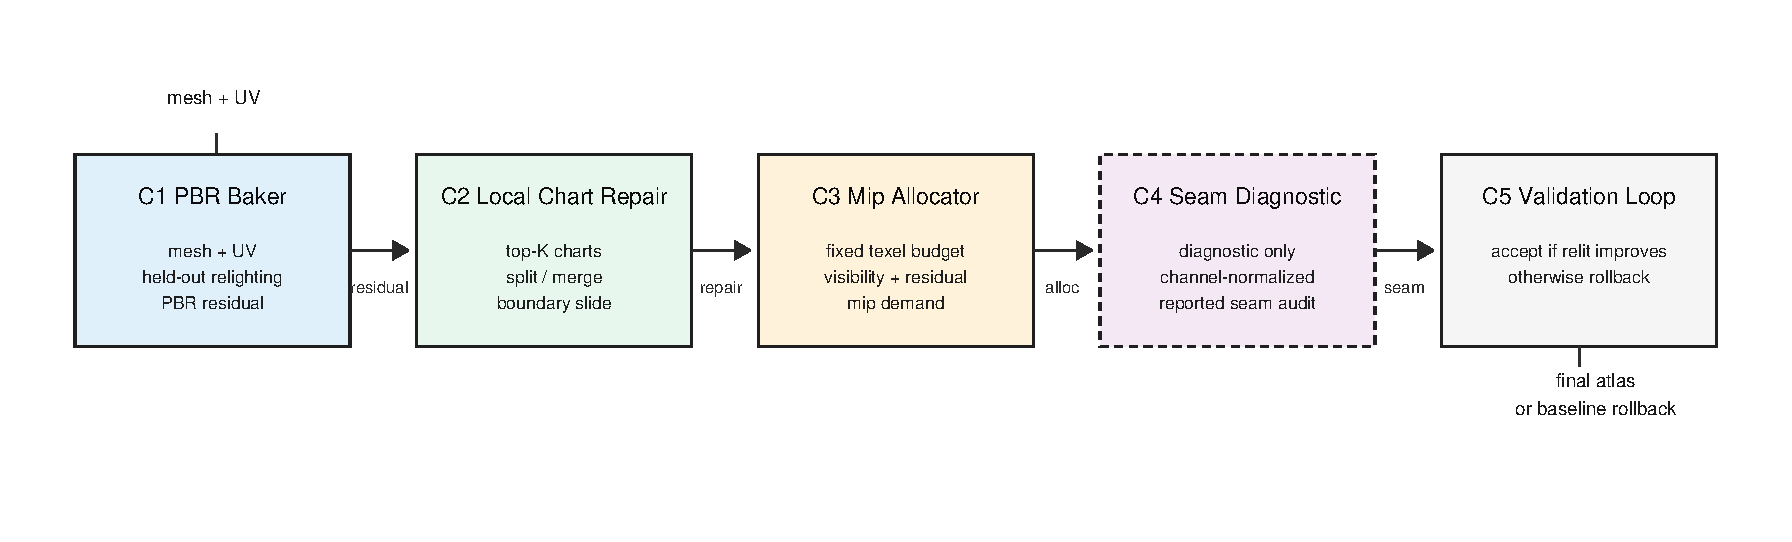
\includegraphics[width=0.95\linewidth]{figures/main/fig2_architecture.pdf}
  \caption{C1--C5 architecture for residual-driven atlas repair. The differentiable PBR baker attributes held-out relighting residuals, C2 edits only local charts, C3 reallocates a fixed texel budget, C4 checks cross-channel seam behavior, and C5 deploys either the accepted atlas or the rolled-back baseline.}
  \label{fig:architecture}
\end{figure}

% === fig3_comparison ===
\begin{figure}[t]
  \centering
  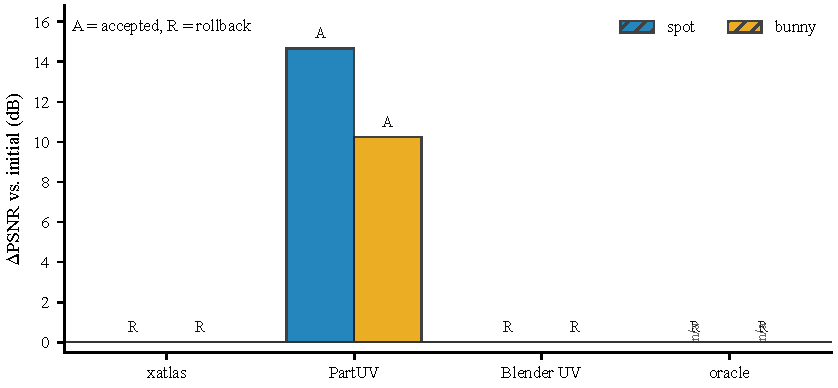
\includegraphics[width=0.95\linewidth]{figures/main/fig3_comparison.pdf}
  \caption{Main B3 comparison on spot and bunny. Positive bars indicate deployed PSNR gain over the initial atlas; labels show whether the C5 gate accepted the repair or rolled back to the baseline.}
  \label{fig:main_comparison}
\end{figure}

% === fig4_ablation ===
\begin{figure}[t]
  \centering
  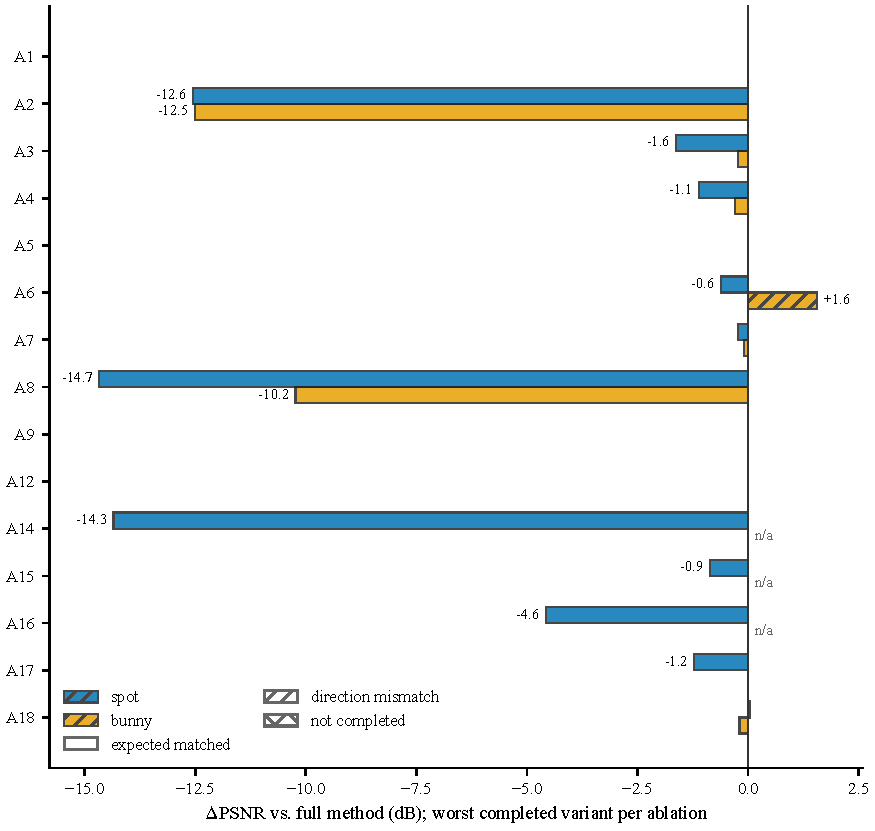
\includegraphics[width=0.95\linewidth]{figures/main/fig4_ablation.pdf}
  \caption{B4 ablation effects measured as PSNR change relative to the full method. Hatching marks expected-direction mismatches or missing completed metric rows, exposing the strong PBR-channel signal and weak or zero-signal components.}
  \label{fig:ablation}
\end{figure}

% === fig5_matched ===
\begin{figure}[t]
  \centering
  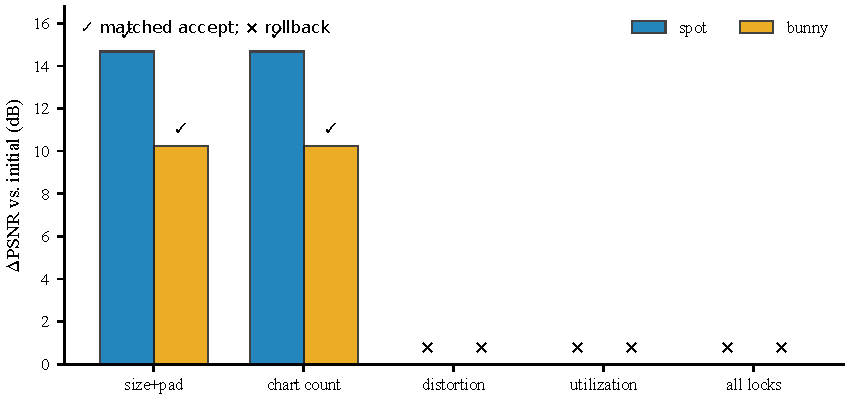
\includegraphics[width=0.95\linewidth]{figures/main/fig5_matched.pdf}
  \caption{Strict matched controls for the accepted PartUV cases. Gains persist when atlas size, padding, or chart count are locked, but vanish under distortion, utilization, or all strict matched controls, indicating a principled downstream-fidelity trade-off.}
  \label{fig:matched_control}
\end{figure}

% === fig6_robustness ===
\begin{figure}[t]
  \centering
  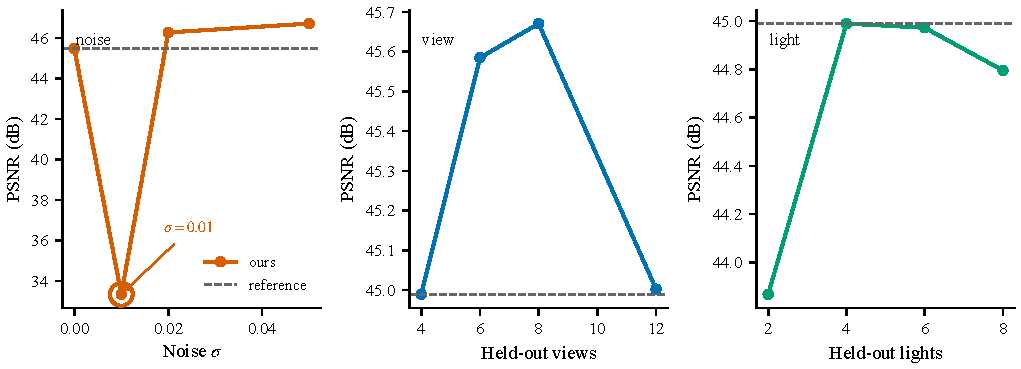
\includegraphics[width=0.95\linewidth]{figures/main/fig6_robustness.pdf}
  \caption{Robustness sweeps for the spot/PartUV accepted case. Light and view sweeps remain stable, while the noise sweep keeps the non-monotonic sigma=0.01 rollback anomaly rather than smoothing it away.}
  \label{fig:robustness}
\end{figure}
